\documentclass{beamer}
\usepackage{simplebeamer}

\begin{document}

%--------------------------------------------------
\section{Why this project?}
%--------------------------------------------------

\begin{frame} \frametitle{}

    \begin{center}
        % \textcolor{LANLBlue}{\textbf{My summer project}}
        \titletext{Coalescent inference of HIV transmission history}

        \vfill
        \small{20 July 2022}

        \vfill
    \end{center}

    %\ftnA{LA-UR-XX-XXXXX} % add this back in when I get an LA-UR

\end{frame}

\begin{frame} \frametitle{\insertsection}

    \begin{itemize}
        \item Prevalence of HIV
        \item Supplementing contact tracing
    \end{itemize}

\end{frame}

%--------------------------------------------------
\section{}
%--------------------------------------------------

\begin{frame} \frametitle{\insertsection}

    Coalescent rate is:
    \[
        \lambda = \frac{k (k-1)}{2 N}
    \]

\end{frame}

%--------------------------------------------------
\section{Results}
%--------------------------------------------------

\begin{frame} \frametitle{\insertsection}

    Main findings:
    \begin{itemize}
        \item First
        \item Second
    \end{itemize}

\end{frame}

\begin{frame} \frametitle{\insertsection}
    \centering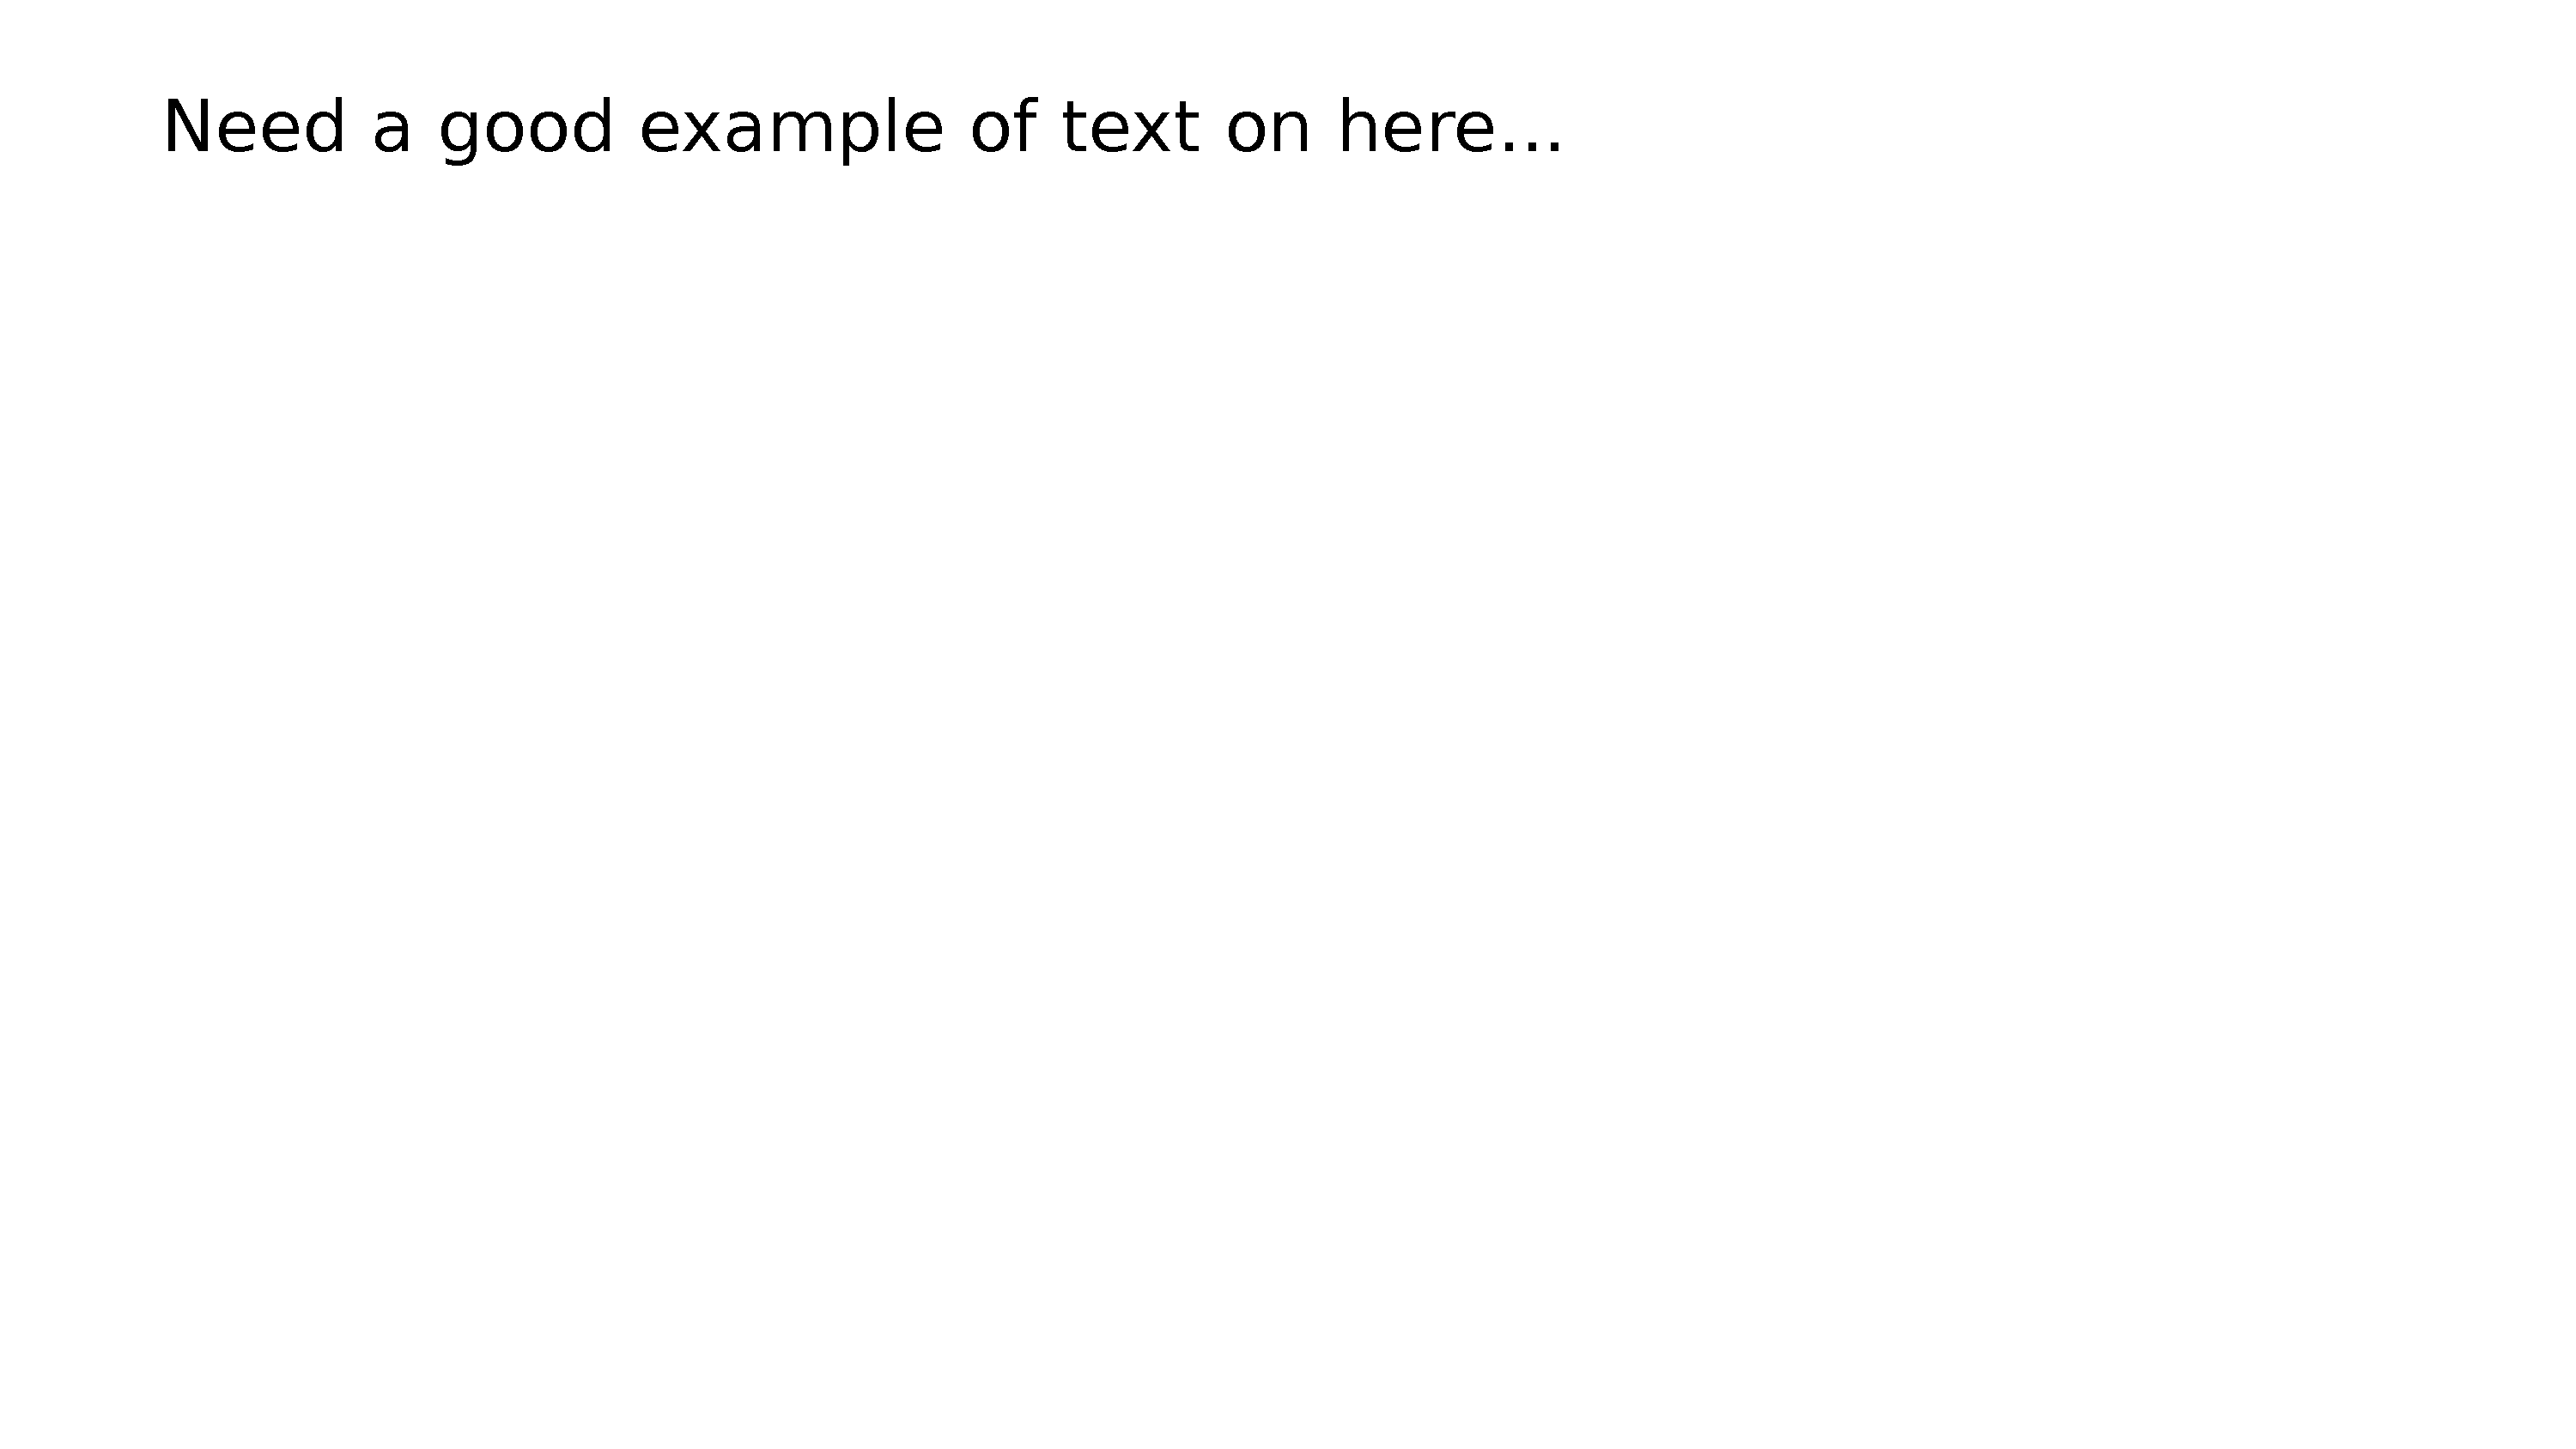
\includegraphics[width=0.8\textwidth]{images/example}
\end{frame}

%--------------------------------------------------
\section{Conclusions}
%--------------------------------------------------

\begin{frame} \frametitle{\insertsection}

    Parting thoughts\ldots

\end{frame}

\end{document}
